%%%%%%%%%%%%%%%%%%%%%%%%%%%%%%%%%%%%%%%%%%%%%%%%%%%%%%%%%%%%%%%%%%%%%%%%%%%%%%%%
\section*{Abstract}
In whole-body control, joint torques and external forces need to be estimated
accurately. In principle, this can be done through pervasive joint-torque
sensing and accurate system identification. However, these sensors are expensive
and may not be integrated in all links. Moreover, the exact position of the
contact must be known for  a precise estimation. If contacts occur on the whole
body, tactile sensors can estimate the contact location, but this requires a
kinematic spatial calibration, which is prone to errors. Accumulating errors may
have dramatic effects on the system identification. As an alternative to
classical model-based approaches we propose a data-driven mixture-of-experts
learning approach using Gaussian processes. This model predicts joint torques
directly from raw data of tactile and force\slash torque sensors. We compare our
approach to an analytical model-based approach on real world data recorded from
the humanoid \robot{}. We show that the learned model accurately predicts the
joint torques resulting from contact forces, is robust to changes in the
environment and outperforms existing dynamic models that use of force\slash
torque sensor data. %\end{abstract}

%%%%%%%%%%%%%%%%%%%%%%%%%%%%%%%%%%%%%%%%%%%%%%%%%%%%%%%%%%%%%%%%%%%%%%%%%%%%%%%

\section{Introduction}\label{sec:introduction}

A key challenge for torque-controlled humanoid robots is to accurately estimate
their dynamics in presence of contacts, e.g., during manipulation in clutter
\cite{Jain2013clutter}, whole-body movements \cite{Handbook2008legged} or ground
contacts in locomotion~\cite{Calandra2014}. Analytic dynamics models suffer from
inaccurate parameter estimation, unmodeled dynamics (e.g., friction, couplings,
elasticities) and noisy sensor measurements. With contacts the problem is even
more challenging due to discontinuities and additional non-linearities, which
are difficult to model or estimate. Moreover, if contact locations are not fixed
a priori or known with sufficient precision, small errors in the localization of
the external force can substantially deteriorate the inverse dynamics
computation~\cite{DelPrete2012}.

Nevertheless, many modern control strategies like inverse dynamics
control~\cite{Erez2012}, computed torque control~\cite{Siciliano2009} or model
predictive control~\cite{Naveau2014} rely on accurate dynamic models. With
inaccurate dynamics models they can produce suboptimal policies by not taking
external forces  into account, which are caused by contacts.

\begin{wrapfigure}{r}{0.3\columnwidth}
%\vspace{-0.5em}
\begin{center}
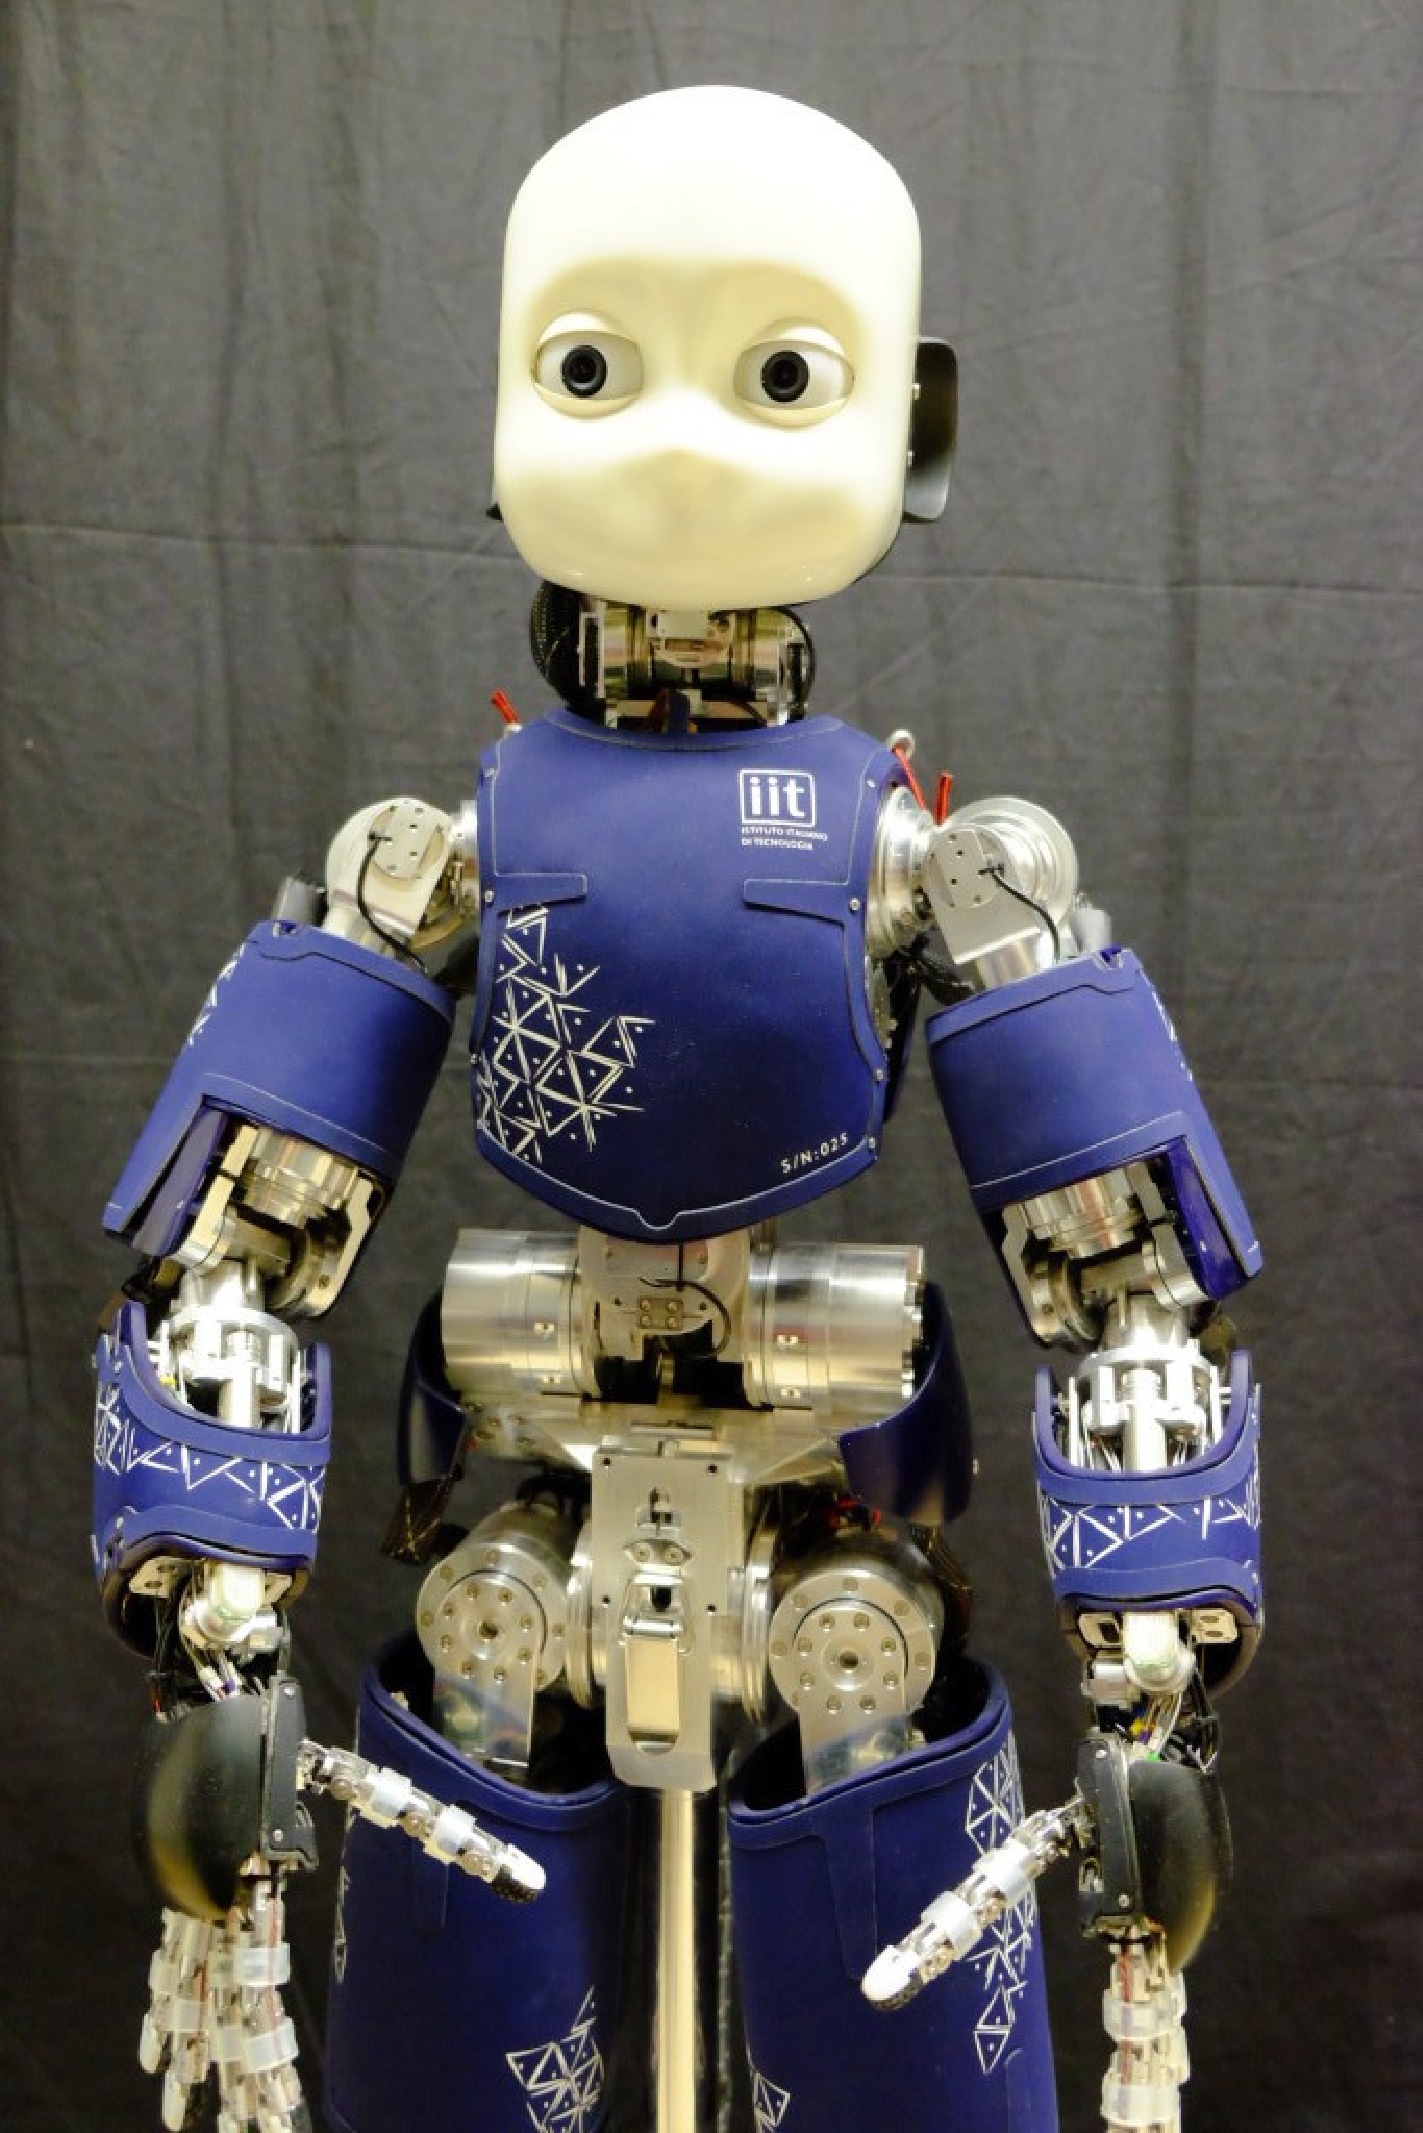
\includegraphics[width=0.29\columnwidth]{robertoICRA/fig/iCubDarmstadt}
\end{center}
\caption{The humanoid robot \textit{iCub} used in the experiments.}
\label{fig:icub}
%\end{figure}
\end{wrapfigure}

As a first step toward a more informed controller that explicitly considers the
effect of contacts, we propose to learn the inverse dynamics model from tactile
sensor readings and force-torque sensors. In contrast to classical techniques
based on the identification of dynamics
parameters~\cite{Yamane2011calibration,Ogawa2014,traversaro2013inertial}, we
propose a fully data-driven machine learning approach based on non-parametric
models, where both the rigid body dynamics as well as the effect of external
forces on the robot structure are learned directly from data collected on the
real robot. The proposed model makes use of the raw sensor data and does not
require a kinematic/dynamics
calibration~\cite{Yamane2011calibration,Ogawa2014,traversaro2013inertial}. In
particular, it does not need a spatially calibrated model of the
skin~\cite{DelPrete2011}. We propose to use a mixtures-of-experts based on
Gaussian Processes (GP) to learn the non-linear system dynamics. Each of these
GP experts models a single contact ``type'' and can be learned
straightforwardly. By using a gating network that activates and deactivates the
individual GP experts we can switch between contact models and generalize to
more complex environments. We evaluate our model learning approach on the arm of
the \robot{} humanoid robot~\cite{Natale2013} (see \fig\ref{fig:icub}) and
compare to a state-of-the-art model-based approach. The learned inverse dynamics
model outperforms the analytic approach and we demonstrate that the learned
model can generalize to changing contact locations. To the best of our knowledge
this is the first demonstration of how joint torques can be learned on a
humanoid robot equipped with tactile and force/torque sensors in presence of
contacts.

%%%%%%%%%%%%%%%%%%%%%%%%%%%%%%%%%%%%%%%%%%%%%%%%%%%%%%%%%%%%%%%%%%%%%%%%%%%%%%%%

\section{Problem Formulation}\label{sec:problem}

The inverse dynamics of a robot with $m$ degrees of freedom can be generally
described by 
\begin{align}
	\torques = \underbrace{\inertiaMatrix\ddq + \Hmatrix}_{\torques_\text{RBD}} + \epsilon\,(\q,\dq,\ddq) \,,
	\label{eq:tau_nocontact}
\end{align}
where $\q$, $\dq$ and $\ddq$ are  the joint positions, velocities and
accelerations, respectively, $\inertiaMatrix$ is the inertia matrix and 
\begin{align*}
	\Hmatrix = C(\q,\dq)\dq + g(\q) + F_v \dq + F_s \,\text{sgn}(\dq) %\in \R^{m \times m}
\end{align*}
is the matrix combining the contributions from Coriolis and centripetal,
friction (viscous and static) and gravity forces. The term
$\epsilon(\q,\dq,\ddq)$ in \eq\eqref{eq:tau_nocontact} captures the errors of
the model, such as unmodeled dynamics (e.g., elasticities and Stribeck
friction), inaccuracies in the dynamic parameters (e.g., masses, inertia),
vibrations, couplings, and sensor noise. With a set $\mathcal{C}=\{c_1 \ldots
c_n\}$ of contacts $c_i$ between the robot and the environment,
\eq\eqref{eq:tau_nocontact} becomes
\begin{align}
	\torques = \underbrace{\inertiaMatrix\ddq + \Hmatrix}_{\torques_\text{RBD}} + \epsilon(\q,\dq,\ddq) + \sum_{c_i \in\mathcal{C}} {\jacobian\T_{c_i}(\q)}\, \extForces_i \, ,
	\label{eq:tau_contact}
\end{align}
where the last term accounts for the additive effect of the external wrenches
(forces and moments) $\extForces_i$ applied at contact location $c_i$, and
$\jacobian_{c_i}(\q)$  is the contact Jacobian. Note that the contact location
$c_i$ is not necessarily fixed as the contacts may occur on the whole robotic
structure and not exclusively at the end-effectors. In such a case, the contact
location, if not known a priori, must be estimated, typically through
distributed tactile sensors. To compute the contact Jacobian, we need the
position of the contact point with respect to the reference frame of the
link~\cite{Fumagalli2012}. Such a knowledge requires a kinematic calibration of
the skin as explained in~\cite{DelPrete2011}.


\subsection{Classical model-based approaches for computing the robot dynamics}

Classical approaches for computing $\torques$ or $\torques_\text{RBD}$ rely on
the dynamics model with known or identified kinematics and dynamics
parameters~\cite{Ivaldi2014}. The torques $\torques_\text{RBD} =
\inertiaMatrix\ddq + \Hmatrix$ can be computed analytically through the rigid
body dynamics model of the robot, a standard parametric description of the
robot~\cite{Featherstone2008}. The term $\epsilon(\q,\dq,\ddq)$ is often
neglected, or implicitly taken into account by considering a perturbation in the
dynamics parameters of $\torques_\text{RBD}$, which need to be identified
accurately.

Although parameter identification for industrial robots is relatively easy with
exciting trajectories~\cite{Pedrocchi2014}, the procedure for floating-base
robots, such as humanoids, is not straightforward because of two main issues: 1)
The generation of sufficiently large accelerations for the identification while
maintaining the robot balance and the control of contacts. This issue was well
explained by Yamane~\cite{Yamane2011calibration}, who proposed a technique to
identify the mass and the local COM of the links in a humanoid robot with fixed
feet at the ground and slow joint trajectories. 2) The measurement of the
external forces $\extForces_i$ exerted on the robot. Note that it may not be
straightforward to measure the external forces~$\extForces_i$ as it is not
possible to cover the robot body with 6-axis force/torque sensors to measure the
force exerted on every possible contact location $c_i$. Usually, such sensors
are big, heavy and expensive. Thus, they are carefully placed where the external
forces are critical for the main tasks. In such a case, it is possible to
identify the dynamics parameters while balancing and walking without additional
contacts~\cite{Ogawa2014}. When force/torque sensors are placed proximally, such
as in the \robot{} arms~\cite{Fumagalli2012}, some of the dynamics parameters
can be identified, but in absence of contacts~\cite{traversaro2013inertial}.

When multiple contacts are exerted on the robot structure at locations other
than the classical end-effectors, it is still possible to compute a precise
inverse dynamics model, but this requires both pervasive joint torque sensing,
such as in \textit{Toro}~\cite{Ogawa2014}, and additional force/torque and
tactile sensing, such as in \robot{}~\cite{Ivaldi2011}. Moreover, it requires
the precise knowledge of the contact locations detected by the tactile sensors,
which necessitates a spatial calibration of the skin~\cite{DelPrete2011}. This
procedure is prone to errors, and it has been shown that small errors in the
kinematics calibration of the taxels (i.e., the tactile units) can induce
non-negligible errors in the estimation of the contact
forces~\cite{DelPrete2012}.

Generally, these model-based approaches have three main limitations: 1) It is
hard to add details about couplings, elasticity, friction and other nonlinear
dynamics, which are required for high accuracy; 2) The performance of the
data-driven identification strongly depends on the experimental setting
(with/without contacts) and the exciting trajectories~\cite{Pedrocchi2014}; 3)
They make strong assumptions to handle contacts.

\subsection{Learning the inverse dynamics}

    \begin{figure}[t]
        \centering
        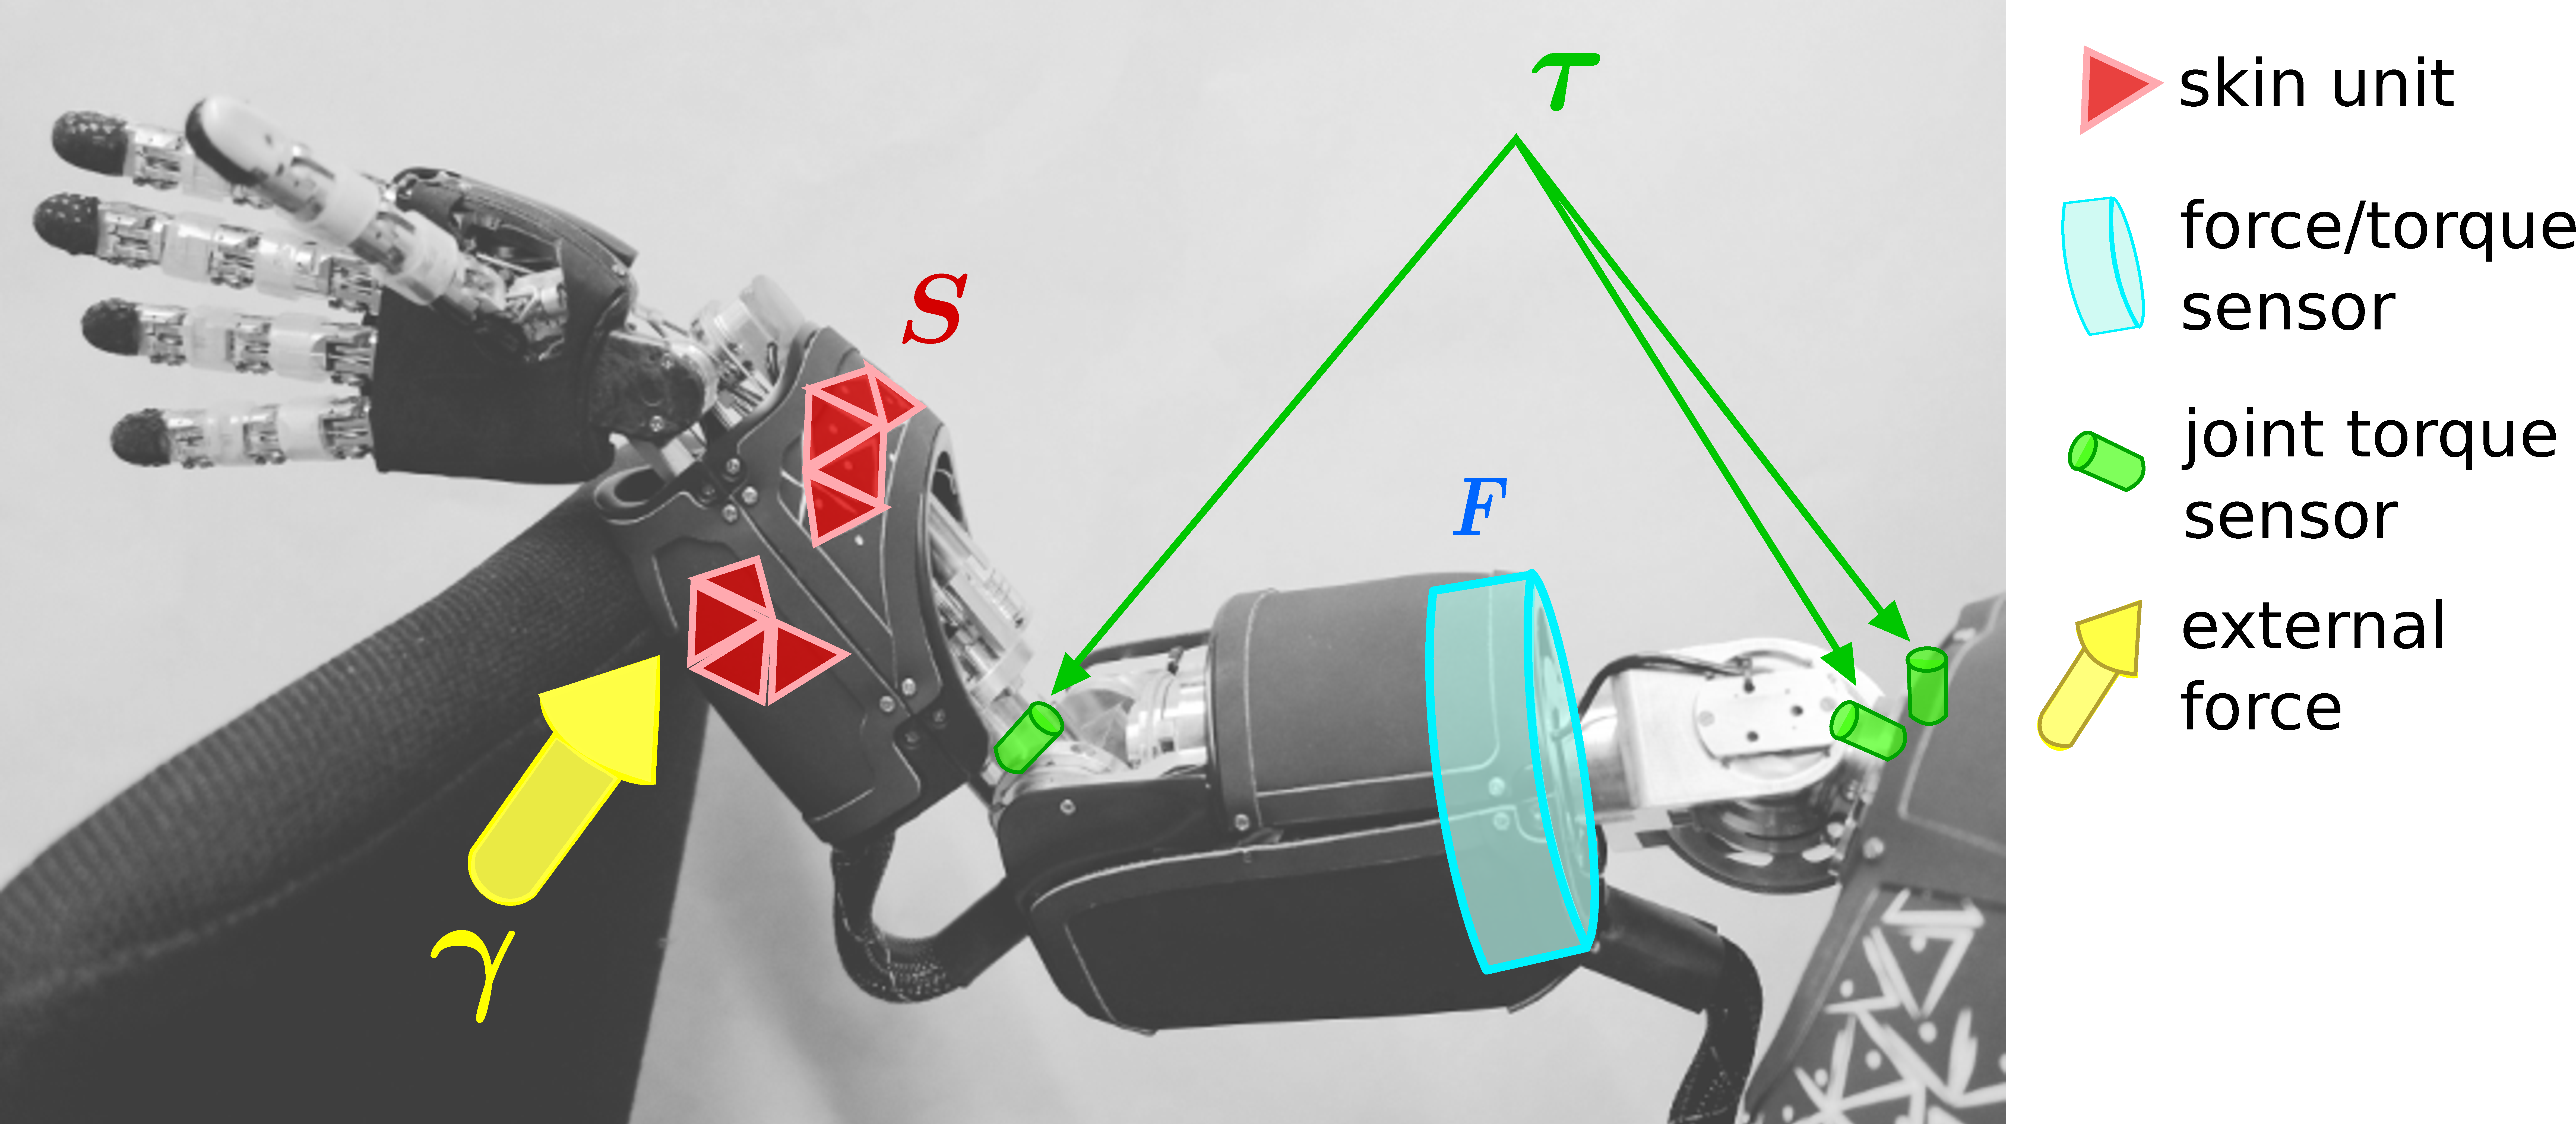
\includegraphics[width=.6\columnwidth]{robertoICRA/fig/concept_gray_new}		
        \caption{Illustration of the force/torque and tactile sensors during a contact of the robot arm with the environment.}
        \label{fig:concept}
        %\figspace
    \end{figure}
An alternative and appealing approach to analytic dynamics computation is to use
machine learning methods to learn the dynamics model of a
robot~\cite{Nguyen-Tuong2008,Vijayakumar2000,Deisenroth2012}. Without the need
for compensating for inaccurate dynamics parameters and accumulated errors, a
learned dynamics model can improve the tracking and control performances of a
robot, as shown in~\cite{Nguyen-Tuong2011} for an industrial manipulator. The
clear advantage of learning the inverse dynamics is that we can overcome the
limitations of the aforementioned approaches: difficulty in modeling complex
nonlinear dynamics, impossibility to generate suitable exciting trajectories,
restrictive assumptions regarding contacts and sensors, prior accurate
kinematics calibration of the tactile sensors. Despite the success of learned
dynamics models in robotics, to the best of our knowledge there are no examples
in the literature where dynamic contacts are also learned. The inclusion of
dynamic contact models in the dynamics highlights two main problems: First,
switching from a no-contact model to a contact-model requires to observe the
system state and to model a discontinuous function~\cite{Toussaint2005}. Second,
switching between different contacts $c_i \in\mathcal{C}$ must be properly
handled.

Here, we provide a first formulation to this problem, and we show that it is
possible to learn the inverse dynamics model of the arm of the \robot{} robot by
means of proximal force/torque measurements~$\ftsForces$ and distributed tactile
sensors~$\skinInput$ (without requiring a spatially calibrated model of the
skin~\cite{DelPrete2011}). 
    
%%%%%%%%%%%%%%%%%%%%%%%%%%%%%%%%%%%%%%%%%%%%%%%%%%%%%%%%%%%%%%%%%%%%%%%%%%%%%%%%%

\section{Learning Inverse Dynamics with Contacts}
\label{sec:mgp}

In this section, we present our proposed approach to learning inverse dynamics
with contacts. We first formalize the problem as learning a mixture-of-experts
model. Then we detail how we implement Gaussian processes as the corresponding
experts.

\subsection{Learning contacts as a mixture-of-experts}
		
\begin{figure}[t]
	\centering
	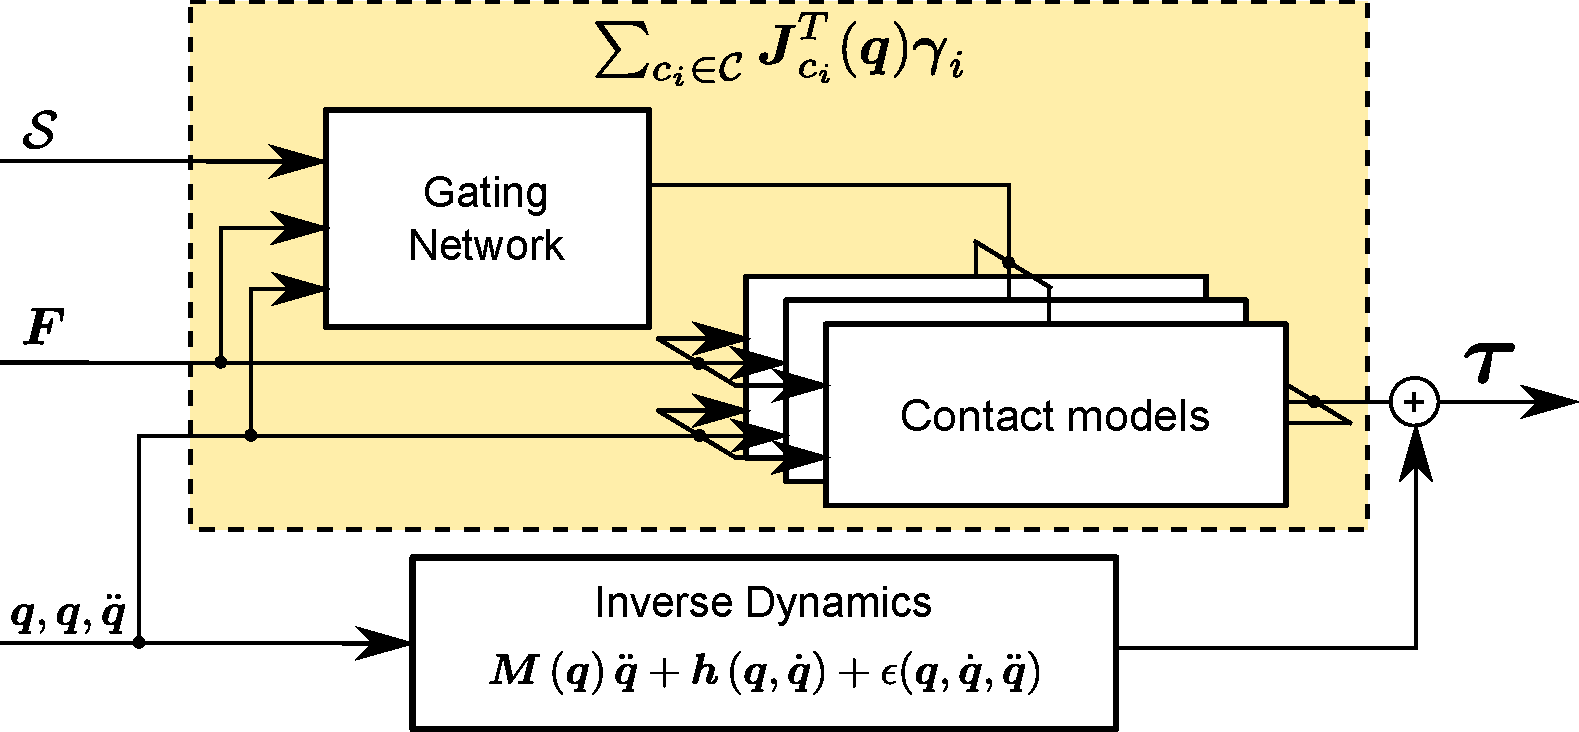
\includegraphics[width =.7\linewidth]{robertoICRA/fig/diagram_2.pdf}
	\caption{Our approach extends existing inverse dynamics without contacts by learning many contact models, which serve as correction terms under different contact types. The decision of which contact model to activate is made by a gating network, which uses skin measurements~$\skinInput$, the force torque sensors~$\ftsForces$ and the current state $\q, \dq, \ddq$.}
	\label{fig:model}
%\figspace
\end{figure}
When learning inverse dynamics with contacts \eq\eqref{eq:tau_contact},
we assume that the (contact-free) inverse dynamics from
\eq\eqref{eq:tau_nocontact} can be computed precisely, either from an analytical
model or from a learned model~\cite{Nguyen-Tuong2011}. In our experiments, we
employ a learned GP model as contact-free inverse dynamics. The reason for this
choice are the unmodeled dynamics $\epsilon\,(\q,\dq,\ddq)$, which introduce
substantial errors even without contacts. As a result of the pre-existing
contact-free inverse dynamics, only the model of the residual term of the
external forces $\sum_{c_i \in\mathcal{C}} {\jacobian\T_{c_i}(\q)}\,
\extForces_i$ has to be separately learned. In this paper, we consider a robot
that is provided with skin measurements~$\skinInput$ from the tactile sensors,
force measurements~$\ftsForces$ from the force torque sensors (FTS) and the
ground truth of the torques~$\torques$ from the joint torque sensors (JTS). An
illustration of these relevant components is shown in \fig\ref{fig:concept}.
Modeling the external forces $\sum_{c_i \in\mathcal{C}}
{\jacobian\T_{c_i}(\q)}\, \extForces_i$ can be formalized as the regression task
\begin{align}
	\outputMatrix = \regressionNo([\q, \skinInput]) + \noise\,,
	\label{eq:regression}
\end{align}   
where $\outputMatrix = \sum_{c_i \in\mathcal{C}}
{\jacobian\T_{c_i}(\q)}\, \extForces_i$ and  $\noise$ is an i.i.d. Gaussian
measurement noise with mean~$0$ and variance~$\sigma_\noise^2$. Contacts with
different parts of the body lead to different effects in the dynamics.
Intuitively, it is necessary to consider the skin input~$\skinInput$ to identify
the position of the contact. Additionally, measurements of the force applied by
the contacts are necessary to deal with a non-static environment. Theoretically,
these measurements can be provided by the skin. However, the artificial skin
used in our experiments does not provide a precise six-dimensional measure of
the contact force. Therefore, in the implementation of our model we substitute
the force measurement from the skin with the force/torque
measurements~$\ftsForces$. The corresponding regression problem
\eq\eqref{eq:regression} is complicated due to the high-dimensional space of the
input $\inputMatrix \in \inputSpace$ (the skin measurements~$\skinInput$ alone
account for hundreds of dimensions). Therefore, we rephrase this regression task
as a problem of learning a mixture-of-experts model. With this model, we
decompose \eq\eqref{eq:regression} as
\begin{align}
	\sum\nolimits_{c_i \in\mathcal{C}} {\jacobian\T_{c_i}(\q)}\, \extForces_i \,=\, \sum\nolimits_{j\in\mathcal{J}} f_j([\q, \ftsForces]) + \noise\,,
	\label{eq:expertofmixtureregression}
\end{align}  
where $\mathcal{J}$ is the set of active experts~$f_j$. Note that the skin
input~$\skinInput$ is no longer explicitly part of the inputs of the experts.
Therefore, each single expert~$f_j$ is now sufficiently low-dimensional to be
modeled independently. At the same time the possibility of summing the
contribution of each contact allows to account for complex behaviors. As single
expert~$f_j$ we use Gaussian processes for the mapping $[\q, \ftsForces] \mapsto
{\jacobian\T_j(\q)} \extForces_j$. A gating network is used to select the
experts that are currently active and to add their contributions.    An
illustration of our approach is shown in \fig\ref{fig:model}. In this paper, we
implement this gating network as a multi-class classifier $\mathcal{J} = g(\q,
\skinInput,\ftsForces)$ that selects which contact is currently ongoing. For
simple tasks, this gating network can be designed using heuristics (e.g., using
thresholds on the activation of the tactile sensors). However, for more complex
systems an adaptive, data-driven approach may be more suitable. In the
experimental section we evaluate the learning of such gating network.

\subsection{Gaussian processes as expert models}

Gaussian Processes (GPs)~\cite{Rasmussen2006} are a state-of-the-art regression
method. They have been used in robotics to learn dynamics
models~\cite{Deisenroth2012} and for control~\cite{Deisenroth2014}. In this
paper, a GP is a distribution over inverse dynamics models \mbox{$f \sim \GP
\left( m_f,k_f \right) \,,$} fully defined by a prior mean~$m_f$ and a
covariance function~$k_f$. We choose as prior mean $m_f \equiv
\torques_\text{RBD}$ and as covariance function~$k_f$ the squared exponential
with automatic relevance determination and Gaussian noise
\begin{align*}
	{k(\vec x_p,\vec x_q)} &= \sigma_f^2\exp\left(\!-\!\tfrac{1}{2}(\vec x_p\! -\!\vec x_q)^T {\mat \Lambda\inv} (\vec x_p \!-\! \vec x_q)\right) \!+\! \sigma_\noise^2\delta_{pq}
\end{align*}
where ${\mat \Lambda}=\diag([l^2_1,...,l^2_D])$ and $\delta_{pq}$ is the
Kronecker delta (which is one if $p=q$ and zero otherwise). Here, $l_i$ are the
length-scales, $\sigma^2_f$ is the variance of the latent function $f(\cdot)$
and $\sigma^2_\noise$ the noise variance. 

In our experiments, when learning contact models, the input is defined as
$\parameters = [\q,\ftsForces]$, while the output (observations) $\vec y =
\torques$ are the torques. Hence, given $n$ training inputs $\mat
X=[\parameters_1,...,\parameters_n]$ and corresponding training targets $\mat
y=[ y_1,..., y_n]$, we define the training data set $\dataset = \{\mat X,\mat
y\}$. Training the GP corresponds to finding good hyperparameters $\vec \theta =
[l_i, \sigma_f, \sigma_\noise]$, which is done by the standard procedure of
maximizing the marginal likelihood~\cite{Rasmussen2006}.   

The GP yields the predictive distribution over torques for a new input $\vec x_* = [\vec q_*, \mat F_*]$
\begin{align}
	&\prob(\vec y|\dataset,\parameters_*,\vec \theta) = \gauss{\mu(\parameters_*)}{\sigma^2(\parameters_*)}\,, 
	\label{eq:one-step prediction distr}
\end{align}
where the mean~$\mu(\parameters_*)$ and the variance~$\sigma^2(\parameters_*)$ are 
\begin{align}
	&\mu(\parameters_*) = \vec k^T_*\vec K^{-1} \mat y\,,\quad \sigma^2(\parameters_*) = k_{**}-\vec k^T_*\mat K^{-1}\vec k_*\,,
	\label{eq:one-step prediction mean and covariance}
	%\label{eq:one-step prediction cov}
\end{align}
respectively. The entries of the matrix $\vec K$ are  $K_{ij}=
k(\parameters_i,\parameters_j)$, and we define
$k_{**}=k(\parameters,\parameters)$ and $\vec k_{*}=k(\vec X,\parameters)$.

	
%%%%%%%%%%%%%%%%%%%%%%%%%%%%%%%%%%%%%%%%%%%%%%%%%%%%%%%%%%%%%%%%%%%%%%%%%%%%%%%%%

\section{Experimental Set-up and Evaluation}
\label{sec:results}


	\begin{figure}[t]
		\centering
		\begin{subfigure}[t]{0.48\hsize}
			\centering
			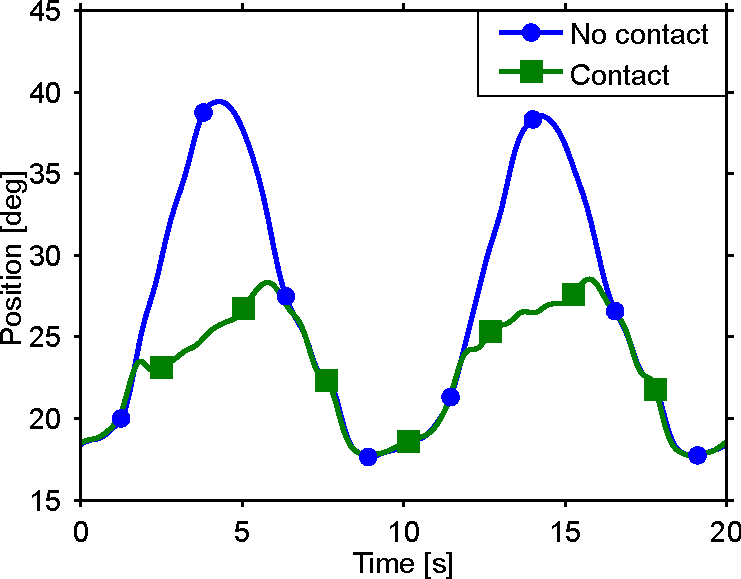
\includegraphics[height=3.2cm]{robertoICRA/fig/exp1_effectContactQ}%[width=.99\columnwidth]{fig/exp1_effectContactQ}
			\caption{Task space}
			\label{fig:exp1:effects_contact:a}
		\end{subfigure}
		\hfill
		\begin{subfigure}[t]{0.48\hsize}
			\centering
			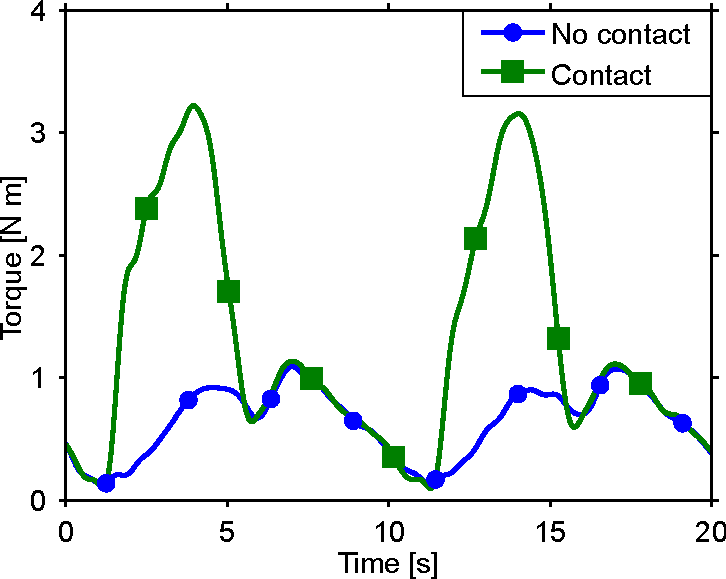
\includegraphics[height=3.2cm]{robertoICRA/fig/exp1_effectContactT}
			\caption{Torque}
			\label{fig:exp1:effects_contact:b}
		\end{subfigure}
		\caption{\textbf{Learning a single contact:} Effects of a contact (green curve) compared to the free movement without obstacle (blue curve). 
		These effects are visible in the task space position~\subref{fig:exp1:effects_contact:a} and in the torque measured by the joint torque sensor~\subref{fig:exp1:effects_contact:b}.}
		\label{fig:exp1:effects_contact}
	\end{figure}
	%


In this section, we describe the experimental setting and the humanoid robot~\robot{} used in the experiments.
We present four different experiments where we demonstrate that
1) Our approach can learn single contact models;
2) A single learned model (i.e., an expert) is robust to small changes in the position of the contact;
3) Our approach extends to multiple contacts by combining models of single contacts;
4) The gating network activating the experts can be learned to reduce the complexity of manually design it.

\subsection{Experimental set-up}

The experiments were conducted on the \robot{}~\cite{Natale2013}, a
humanoid robot with 53 degrees of freedom, sized as a child (104 cm tall, 24 kg
of weight). This robot is equipped with several sensors: an inertial sensor in
the head, four 6-axis force/torque sensors placed proximally in the middle of
legs and arms, and an artificial skin consisting of many distributed tactile
elements (taxels) mounted on the robot covers~\cite{Cannata2008}. The
information from these three types of sensors is used to estimate the joint
torques and the external contact forces by the \idyn{} 
library~\cite{Ivaldi2011}. In the following, $\torques_{\rm IDYN}$ denotes the
joint torques estimated by the \idyn{} library, which we use as analytical model
for comparison. For more detail on its contact detection and taxels calibration
we refer to~\cite{DelPrete2011,DelPrete2012}.
	
 
The \robot{} used in the experiments is equipped with three additional Joint
Torque Sensors (JTSs), two in the shoulder and one in the elbow. The JTSs are
calibrated by computing the offset and gain trough least-square regression with
respect to the output of~\idyn{}. We consider these calibrated JTSs as ground
truth measurements of the joint torques~$\jtsForces$. In our experiments, we
used the \robot{} torso and arms (3 and 7 degrees of freedom, respectively) and
the skin input~$\skinInput$ from the forearm, which consists of 270 sensor
measurements.

	\begin{figure}[t]
		\centering
		\begin{subfigure}[t]{0.48\hsize}
			\centering
			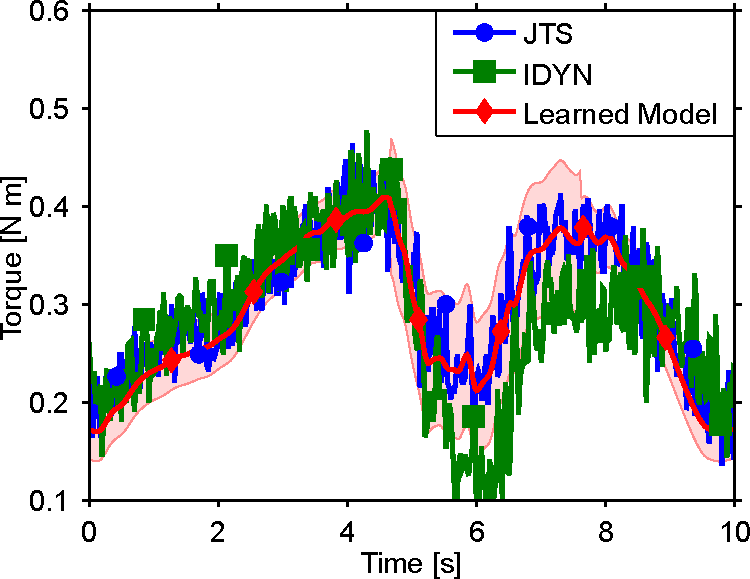
\includegraphics[width=.69\columnwidth]{robertoICRA/fig/exp1_model_notfilt}
			\caption{Real data.}
			\label{fig:exp1:model_contact:a}
		\end{subfigure}
		\hfill
		\begin{subfigure}[t]{0.48\hsize}
			\centering
			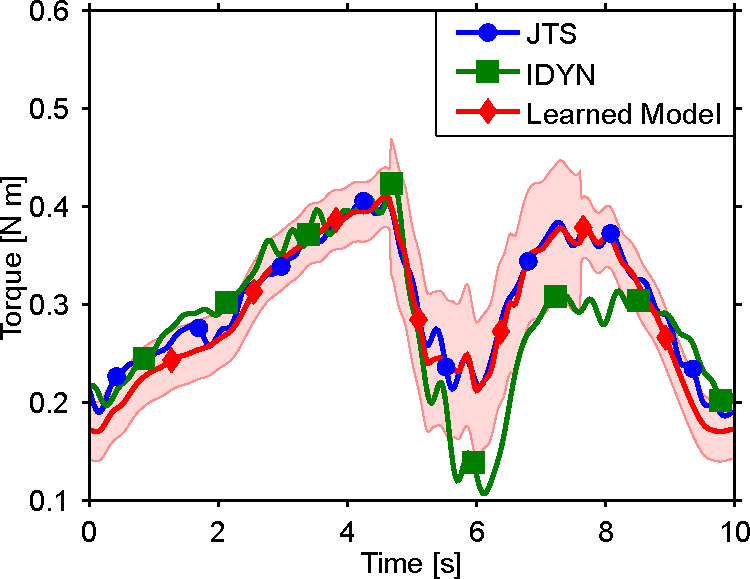
\includegraphics[width=.69\columnwidth]{robertoICRA/fig/exp1_model_filt}
			\caption{Filtered visualization.}
			\label{fig:exp1:model_contact:b}
		\end{subfigure}
		\caption{\textbf{\nameref{sec:results:exp1}}: Comparison of the torque measured at the elbow (with contact) by the JTS,  estimated by \idyn{} and our learned model (shown as $\text{mean}\pm 2\,\text{std}$). 
		Our learned model better predict the torque measured by JTS~\subref{fig:exp1:model_contact:a}.
		Additionally, due to the identification of the noise in the model, its prediction is smoother compared to both the noisy JTS measurements and the prediction from \idyn{}.
		For visualization purposes we also show the predictions when filtering JTS and \idyn{}~\subref{fig:exp1:model_contact:b}.
		}
		\label{fig:exp1:model_contact}
        %\figspace
	\end{figure}
	%
    	% 
	\begin{table}[t]
		\resizebox{\hsize}{!}{
		\centering
		\begin{tabular}{|l|l|c|c|c|}
			\hline 
			& Method	& Shoulder 1 [Nm] & Shoulder 2 [Nm] & Elbow [Nm] \\
% 			\cline{2-7}
			\hline 	
			\multirow{2}{*}{Full trajectory}  & \idyn{} & $0.09 \pm 1.1 \times 10^{-3}$ & $0.16 \pm 1.8 \times 10^{-3}$ & $0.05 \pm 7.4\times 10^{-4}$ \\ 
			& Our model 		& $\mathbf{0.04  \pm 5.6 \times 10^{-4}}$ & $\mathbf{0.07  \pm 9.8\times 10^{-4}}$ & $\mathbf{0.02  \pm 3.1\times 10^{-4}}$ \\
			\hline
			\multirow{2}{*}{Contact only}  & \idyn{} 	& $0.07 \pm 3.1 \times 10^{-3}$ & $0.13 \pm 5.7 \times 10^{-3}$ & $0.08 \pm 3.0 \times 10^{-3}$\\ 
			& Our model 		& $\mathbf{0.03  \pm 1.5 \times 10^{-3}}$ & $0.12  \pm 5.9 \times 10^{-3}$ & $\mathbf{0.03  \pm 1.3 \times 10^{-3}}$ \\
			%\cline{2-7}
			\hline
		\end{tabular}
		}
		\caption{\textbf{\nameref{sec:results:exp1}:} Mean and standard deviation of the mean for the RMSE of the test set for ground truth, predictions with the \idyn{} and our learned model. 
		The learned model predicts the torque more accurately than~\idyn{} for both the full trajectory and  during the only contact phase.
		}
		\label{tab:exp1}
        %\figspace
	\end{table}
	%

\subsection{Learning a single contact}
\label{sec:results:exp1}


In this experiment, we consider the \robot{} making contact with a single
obstacle. The evaluation is performed on a simple tracking task with the
\robot{}'s end-effector moving along a circular trajectory. We repeat the task 
twice: first without any contact and then with a contact at a fixed position.
\fig\ref{fig:exp1:effects_contact} shows the effects of the contact in terms of
position and torque during the tracking task. When the contact occurs the
position error increases considerably. As a result, the torque is increased to
compensate for the obstacle. We collected 10 repetitions of the trajectory with
the contact and used 8 of them to train the model. The remaining trajectories
are used as test set to evaluate the predictive performances of our learned
model. For this experiment we consider a single expert (the gating network still
decides whether to activate the expert).
    
    
	We compare the baseline joint torque (measured by the JTS) to the joint torque estimated by the analytic model \idyn{} and  the joint torque $\torques_\text{IDM}$ predicted by our learned model.
	In \tab\ref{tab:exp1}, we report the root mean square error (RMSE) and the standard deviation of the mean of \idyn{} and our learned model for all the three joints.
	Additionally, we report both the error of the learned models (learned RBD plus learned contact model) during the full trajectory and exclusively \textit{during} the contact. 
	In five out of six cases, the learned model performs better than the analytic model. 
    In the sixth case (contact only, shoulder 2), the performance of the learned model is similar to the analytic model.
    However, increasing the amount of data used for training may further increase the performance of the learned model. 
	A visual representation of the predictions of the test set for the elbow joints is shown in~\fig\ref{fig:exp1:model_contact}.
	
    This experiment provides evidence that the classical rigid-body dynamics model $\torques_\text{RBD}(\q,\dq,\ddq)$ and the \idyn{} estimation (that also exploits proximal force/torque sensing) fail to accurately estimate the joint torques when the robot is in contact with the environment. 
	Moreover, we show that the learned contact model, when combined with the RBD model, provides a better approximation of the joint torque.
	
\subsection{Robustness of the single contact model}
\label{sec:results:exp2}

	%
	\begin{figure}[t]
		\resizebox{\hsize}{!}{
		\centering
		\begin{subfigure}[t]{0.48\hsize}
			\centering
			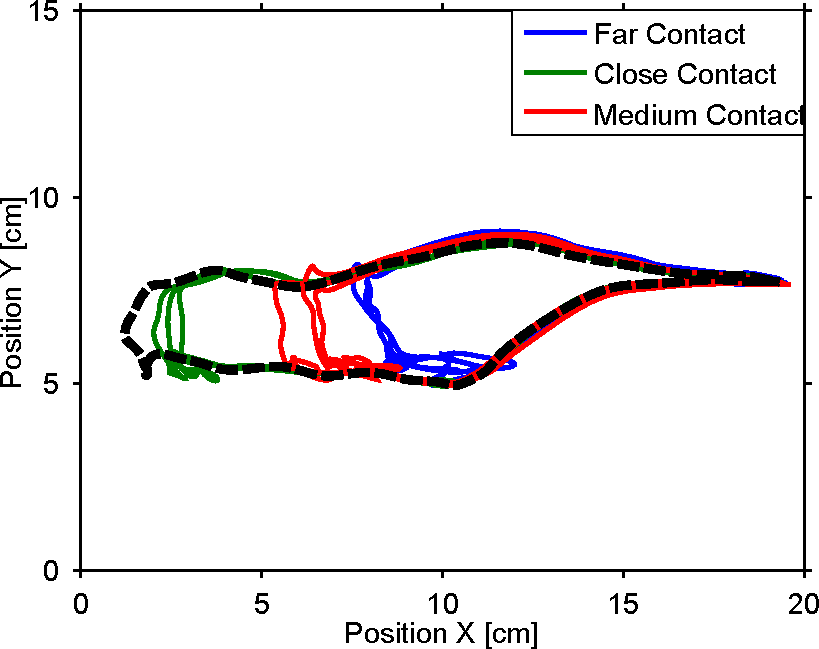
\includegraphics[height=4.2cm]{robertoICRA/fig/generalized_contact_a.pdf} %[width=.99\columnwidth]
			\caption{Task space}
			\label{fig:effects_contact:a}
		\end{subfigure}
		\hfill
		\begin{subfigure}[t]{0.48\hsize}
			\centering
			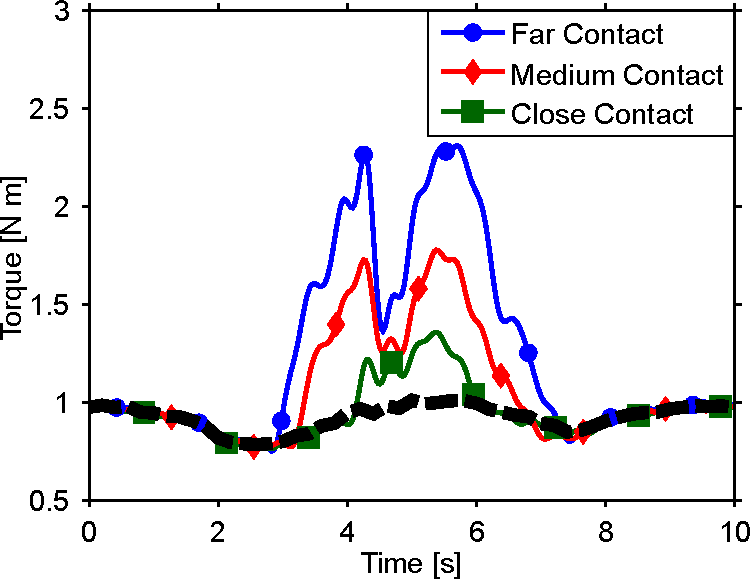
\includegraphics[height=4.2cm]{robertoICRA/fig/generalized_contact_b.pdf} % [width=.99\columnwidth]
			\caption{Torque}
			\label{fig:effects_contact:b}
		\end{subfigure}
		}
		\caption{\textbf{\nameref{sec:results:exp2}:} Effects of the contact on the task space and the torque for the three different contact types: contact 1 (far), contact 2 (medium) and contact 3 (close). 
		The task in absence of contact is displayed as reference (\textbf{black dashed curve}). 
		%\comment{Figures generated by \textit{Figures\_exp2}}
		}
		\label{fig:exp2:effects_contact}
        %\figspace
	\end{figure}
	%
	
	In the following, we show that the prediction performance of each GP expert is robust to small variations in the position of the contact.
	This is important since the exact position of the obstacle does not need to be known in advance (within a single expert $f_j$).
	As in the previous experiment we consider a tracking task along a circular trajectory.
	However, this time the obstacle is placed at one of three different positions along the trajectory: close, medium and far.
    Each of these obstacles is shifted 2\,cm along the horizontal axis.
	Obstacles at different positions along the trajectory lead to different effects in terms of both joint position and torque signal, as clearly visible in~\fig\ref{fig:exp2:effects_contact}.
	Note that the skin input~$\skinInput$ will also be affected, as shown in~\fig\ref{fig:exp2:skin}. 
    Hence, we could potentially learn a separate expert for each contact. 
    However, we only consider a single expert as we want to demonstrate the robustness of a single expert, not of the gating network.
    
    
	\begin{figure}[t]
		\centering
		\begin{subfigure}[t]{0.30\hsize}
        \centering
			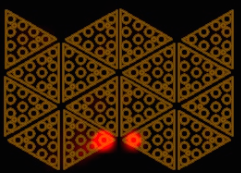
\includegraphics[height=1.8cm]{robertoICRA/fig/paris2_new} 
			\caption{Contact 1}
		\end{subfigure}
		\hspace{0.1cm}
		\begin{subfigure}[t]{0.30\hsize}
        \centering
			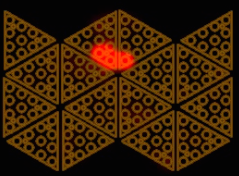
\includegraphics[height=1.8cm]{robertoICRA/fig/paris3_new} 
			\caption{Contact 2}
		\end{subfigure}
		\hspace{0.1cm}
		\begin{subfigure}[t]{0.30\hsize}
        \centering
			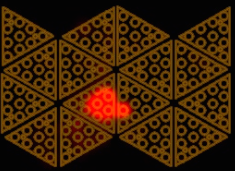
\includegraphics[height=1.8cm]{robertoICRA/fig/paris7_new}
			\caption{Contact 3}
		\end{subfigure}
		\caption{\textbf{\nameref{sec:results:exp2}}. The different contact locations detected by the forearm skin respectively for the three contacts: contact~1 (far), contact~2 (medium) and contact~3 (close).}
		\label{fig:exp2:skin}
        %\figspace
	\end{figure}
	%

	% 
	\begin{table}[t]
		\resizebox{\hsize}{!}{
		\centering
		\begin{tabular}{|l|l|c|c|c|}
			\hline 
			& Method	& Shoulder 1 [Nm] & Shoulder 2 [Nm] & Elbow [Nm] \\
			\hline 	
			\multirow{2}{*}{Far contact}  & \idyn 	& $0.13 \pm 3.9 \times 10^{-3}$  &  $0.40 \pm 9.7\times 10^{-3}$ & $0.06 \pm 1.9\times 10^{-3}$ \\ 
			&Our model 		& $\mathbf{0.06  \pm 1.9\times 10^{-3}}$ & $\mathbf{0.08  \pm 2.9\times 10^{-3}}$ & $\mathbf{0.03  \pm 8.0 \times 10^{-4}}$\\
			\hline 	
			\multirow{2}{*}{Close contact}  & \idyn 	& $0.09 \pm 2.2\times 10^{-3}$ & $0.22 \pm 4.5\times 10^{-3}$ & $0.04 \pm  0.9\times 10^{-3}$\\ 
			&Our model 		& $\mathbf{0.06  \pm 1.4\times 10^{-3}}$ & $\mathbf{0.06 \pm 1.4\times 10^{-3}}$ & $\mathbf{0.02  \pm 6.3\times 10^{-4}}$ \\ % 0.58 0.58 is correct!
			\hline 	
			\multirow{2}{*}{Medium contact}  & \idyn 	& $0.10 \pm 2.8\times 10^{-3}$ & $0.32 \pm 6.7\times 10^{-3}$ & $0.05 \pm 1.3\times 10^{-3}$ \\ 
			&Our model 		& $\mathbf{0.06 \pm 1.7\times 10^{-3}}$ & $\mathbf{0.12 \pm 4.7\times 10^{-3}}$ & $0.05 \pm 1.7\times 10^{-3}$ \\
			\hline
		\end{tabular}
		}
		\caption{\textbf{\nameref{sec:results:exp2}:} Errors between the ground truth~(JTS) and the predictions with either the \idyn{} and our learned model on the test set. 
		A single expert is robust to small variations of the contact.
		}
		\label{tab:exp2}
        %\figspace
	\end{table}
	%

    The contact model is learned using the data collected from contact 1 and contact 3 (far and close contacts) and as validation the data set generated from the \textit{unseen} contact 2 (medium) is used.
	In \tab\ref{tab:exp2}, the RMSE for all three contacts are reported for \idyn{} and our learned model, respectively.
	The results show that the learned model is robust to unseen contacts and performs  equally well or better than the analytic model \idyn{}. 

\subsection{Learning multiple contacts}
\label{sec:results:exp3}


		% 
	\begin{table}[t]
		\resizebox{\hsize}{!}{
		\centering
		\begin{tabular}{|l|l|c|c|c|}
			\hline 
			& Method	& Shoulder 1 [Nm] & Shoulder 2 [Nm] & Elbow [Nm] \\
			\hline 	
			\multirow{2}{*}{Right contact} & \idyn{} & $0.10\pm 1.3 \times 10^{-3}$ & $0.13\pm 1.6 \times 10^{-3}$ & $0.06\pm 8.1 \times 10^{-4}$ \\ 
			& Our model 		& $\mathbf{0.04\pm 6.3 \times 10^{-4}}$ & $\mathbf{0.07\pm 1.2 \times 10^{-3}}$ & $\mathbf{0.02\pm 2.7 \times 10^{-4}}$ \\
			\hline
			\multirow{2}{*}{Left contact}  & \idyn{} & $0.08 \pm 1.2 \times 10^{-3}$ & $0.16 \pm 2.0 \times 10^{-3}$ & $0.05 \pm 8.2 \times 10^{-4}$ \\ 
			& Our model 		& $\mathbf{0.03 \pm 5.7 \times 10^{-4}}$ & $\mathbf{0.07 \pm 9.6 \times 10^{-4}}$ & $\mathbf{0.02 \pm 2.8 \times 10^{-4}}$ \\
			\hline
			\multirow{2}{*}{Both contacts}  & \idyn{} & $0.10 \pm 1.3 \times 10^{-3}$ & $0.11 \pm 1.4 \times 10^{-3}$ & $0.07 \pm 8.4 \times 10^{-4}$ \\ 
			& Our model 		& $\mathbf{0.05\pm 8.3 \times 10^{-4}}$ & $\mathbf{0.10\pm 1.6 \times 10^{-3}}$ & $\mathbf{0.03 \pm 4.0 \times 10^{-4}}$ \\
			\hline
		\end{tabular}
		}
		\caption{\textbf{\nameref{sec:results:exp3}:} Root mean square error between the ground truth~(JTS) and the predictions with the \idyn{} and our learned model on the test set. 
		Our learned model predicts the torque more accurately than \idyn{}.
		}
		\label{tab:exp3}
        %\figspace
	\end{table}
	%
	%
    After learning single contacts, we now show how to combine the learned models to adapt to unseen and more complex environments with multiple contacts.
	We consider a scenario having the \robot{} performing a circular motion with its left arm.
	We initially performed two experiments with an obstacle either on the left and on the right of the reference trajectory (see \fig\ref{fig:exp3:icuparis_experiment_bars}).
	With the data collected in these two contact cases, we trained two independent expert models $f_1$, $f_2$, one for each contact.
	We repeated the experiment, but this time with both left and right contacts 
    and used this last unseen case to validate our models. 
\fig\ref{fig:exp3:gating} shows an example of the prediction and the corresponding activation of the two contact models. 
	During both the right and the left contact, the corresponding experts are activated by the gating network.
	Therefore, we can successfully combine the contributions of the single contact models learned to generalize to unseen cases with multiple contacts.
	 \tab\ref{tab:exp3} reports the RMSE for the predictions.
     We notice that even in this experiment the experts accurately learn the effects of single contacts.
     Moreover, the gating network allows us to combine the experts to generalize to unseen environments, such as in the case of both contacts. 
   
	\begin{figure}[t]
		\begin{minipage}{.32\linewidth}
			\centering
			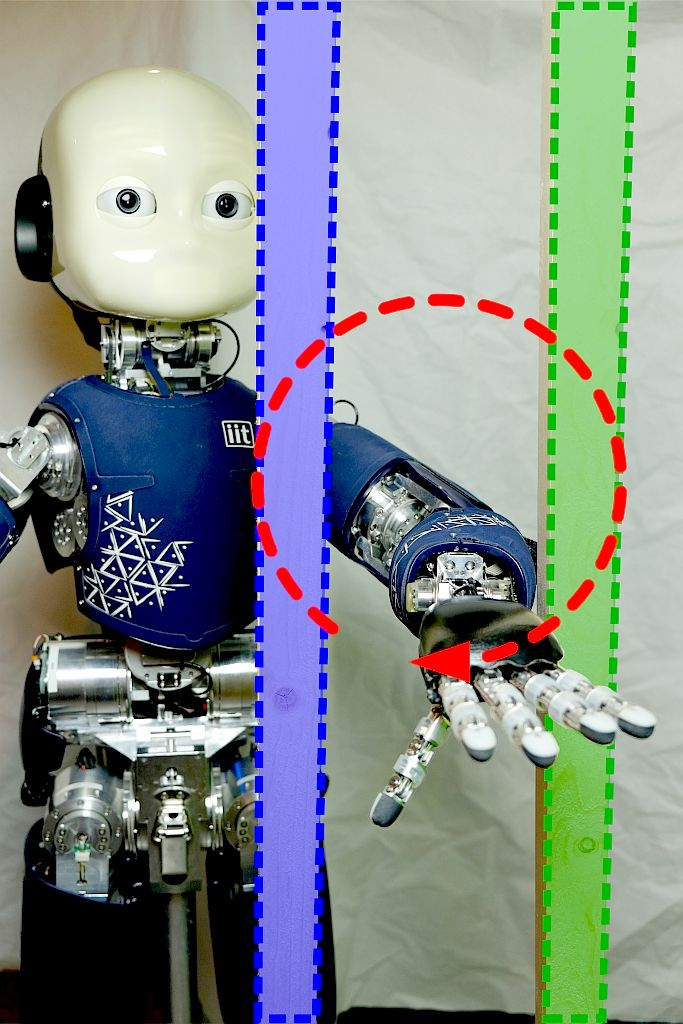
\includegraphics[width =.79\linewidth]{robertoICRA/fig/iCubParis02_Double_Contact}
			\caption{\textbf{\nameref{sec:results:exp3}:} The robot performs a circle with its left arm. 
			The forearm collides alternatively with the left, the right or both contacts.}
			\label{fig:exp3:icuparis_experiment_bars}
		\end{minipage}	
		\hfill
		\begin{minipage}{.52\linewidth}
			\centering
			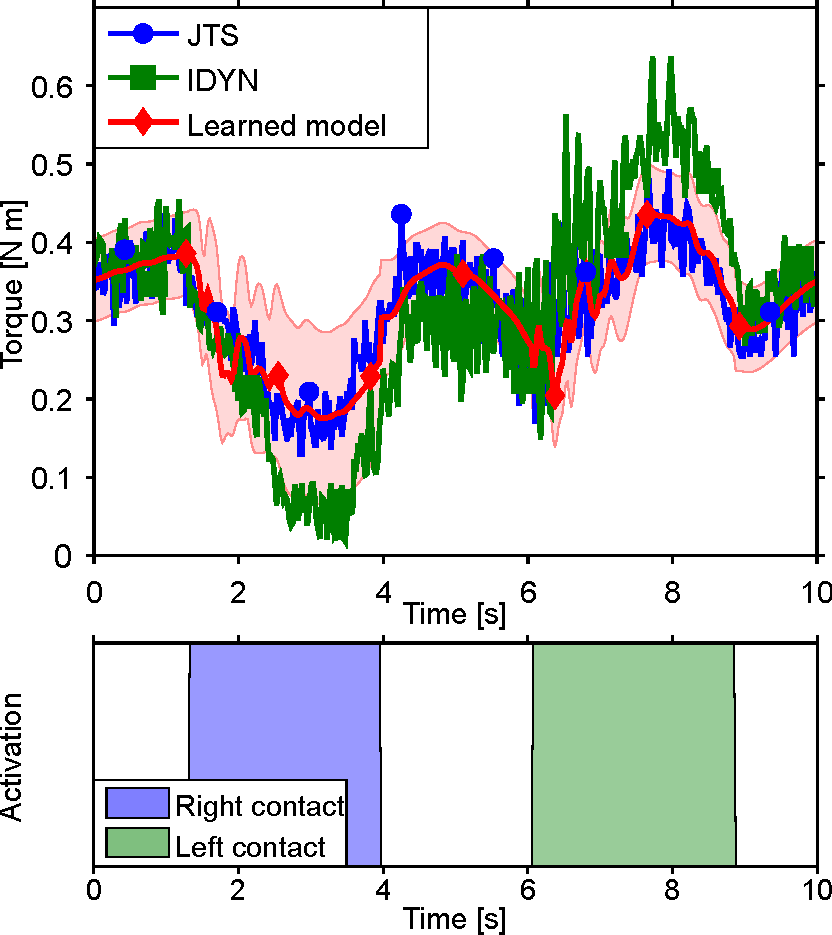
\includegraphics[width=.79\linewidth]{robertoICRA/fig/exp3_both}
			\caption{\textbf{\nameref{sec:results:exp3}:} Prediction of torques with multiple contacts and the corresponding activation of the gating network.
			%Various models are shown, but individually, none of them correctly capture the dynamics of the system. 
			Our mixture-of-experts model combines single-contact models to a multiple-contact model.
			}
			\label{fig:exp3:gating}
		\end{minipage}	
        %\figspace
	\end{figure}

\subsection{Learning the gating network}
\label{sec:results:exp5}

	So far, we assumed a heuristic gating network to select the active experts.
	In this experiment we show that a learned gating network achieves a comparable accuracy as a manually devised heuristic.
    As ground truth to evaluate the performances, as well as for training the classifier, we labeled the data with one of the following labels: no contact, left contact, right contact.
    The heuristic is based on thresholds of the activation of the skin input~$\skinInput$ and the force torque sensors~$\ftsForces$.
	We train a Support Vector Machine (SVM) classifier (using the library LIBSVM~\cite{Chang2011}) having as input $\q, \skinInput, \ftsForces$ and as output the contact labels (none, left, right).

	We evaluated the performance of the trained classifier on an unseen test set.
	\fig\ref{fig:exp5:accuracy} shows that the learned SVM achieved a classification accuracy that is similar to the heuristic gating network. 
    Equivalent results are obtained in terms of RMSE of the inverse dynamics when comparing the experts models learned by the gating networks.
    However, training the gating network (i.e., training the SVM classifier) requires considerably less expert knowledge compared to designing a heuristic. 
    As there is no visible performance difference, we conclude that training the gating network is generally preferable.
Increasing the number of training data may further increase the accuracy of the gating network.



%%%%%%%%%%%%%%%%%%%%%%%%%%%%%%%%%%%%%%%%%%%%%%%%%%%%%%%%%%%%%%%%%%%%%%%%%%%%%%%%

\section{Conclusions}
\label{sec:conclusion}

Whole-body control strategies that exploit contacts need accurate models of the
system dynamics. This is crucial for balance and stabilization, and to increase
the number of potential actions that the robot is able to execute, e.g.,
creating a contact to reach for distant objects. We introduced a data-driven
mixture-of-experts approach based on Gaussian processes  for learning inverse
dynamics models with contacts. We evaluated our model on the \robot{} humanoid
robot using tactile sensors and force/torque sensors as model inputs.  We showed
that the model accurately predicts contact forces and outperforms a
state-of-the-art analytical approach used to estimate the joint torques in
\robot{}. The estimation from the learned model does not rely on dynamic
parameters, but it is completely data-driven and based on tactile sensors and
force/torque sensors. As a result, our approach does not require a spatially
calibrated model of the skin~\cite{DelPrete2011,DelPrete2012}. This is a
promising feature for robust control strategies that explicitly takes contacts
into account. 

	\begin{figure}[t]
			\centering
			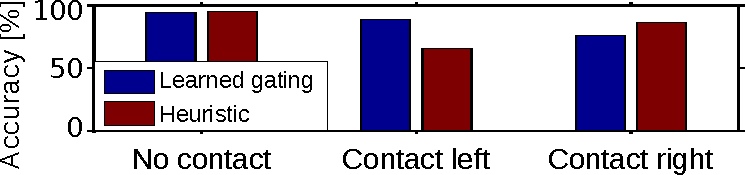
\includegraphics[width=.5\hsize]{robertoICRA/fig/exp5_accuracy_red}
		\caption{\textbf{Learning the gating network:} Classification accuracy for the heuristic and learned SVM gating networks.
		}
		\label{fig:exp5:accuracy}
        %\figspace
	\end{figure}

